\documentclass[UTF8,zihao=-4,a4paper]{ctexart}

\usepackage[left=1.86cm,right=1.86cm,top=1.72cm,bottom=1.78cm]{geometry}
\usepackage{graphicx}
\usepackage{caption}
\usepackage{xcolor}
\usepackage[hidelinks]{hyperref}
\usepackage{fancyhdr}
\usepackage{titlesec}
\usepackage{enumitem}
\usepackage{array,tabularx,booktabs,longtable}
\usepackage{float}
\usepackage{verbatim}

\definecolor{TitleBlue}{HTML}{155E95}
\definecolor{Ink}{HTML}{1F2933}
\definecolor{Muted}{HTML}{596474}
\definecolor{LineGray}{HTML}{D8DEE8}
\definecolor{SoftGray}{HTML}{F6F7F9}
\definecolor{WarmGray}{HTML}{F1F3F5}
\definecolor{Accent}{HTML}{2E6F5E}
\definecolor{LightGreen}{HTML}{EEF7F3}

\hypersetup{
  pdfauthor={陈云海},
  pdftitle={智能联网时钟系统项目交付说明文档}
}

\setlength{\parindent}{2em}
\setlength{\parskip}{0.18em}
\linespread{1.14}
\raggedbottom
\sloppy
\emergencystretch=3em
\setcounter{tocdepth}{0}
\graphicspath{{submission/design_intro_assets/}{design_intro_assets/}}
\captionsetup{font=small,labelfont=bf,labelsep=space,skip=4pt}
\setlist[itemize]{leftmargin=2em,itemsep=0.14em,topsep=0.25em,parsep=0em}
\setlist[enumerate]{leftmargin=2.2em,itemsep=0.14em,topsep=0.25em,parsep=0em}

\titleformat{\section}{\heiti\zihao{-3}\color{Ink}}{\thesection}{0.65em}{}
\titleformat{\subsection}{\heiti\zihao{4}\color{Ink}}{\thesubsection}{0.65em}{}
\titleformat{\subsubsection}{\heiti\zihao{-4}\color{Ink}}{\thesubsubsection}{0.55em}{}
\titlespacing*{\section}{0pt}{1.08em}{0.42em}
\titlespacing*{\subsection}{0pt}{0.76em}{0.26em}
\titlespacing*{\subsubsection}{0pt}{0.46em}{0.18em}

\pagestyle{fancy}
\fancyhf{}
\fancyhead[L]{智能联网时钟系统 v2.2}
\fancyhead[R]{524031910102\quad 陈云海}
\fancyfoot[C]{\thepage}
\renewcommand{\headrulewidth}{0.25pt}
\setlength{\headheight}{15pt}

\newcommand{\keypoint}[1]{\textbf{#1}}
\newcommand{\code}[1]{\texttt{\detokenize{#1}}}

\newenvironment{infobox}[1]{%
  \par\vspace{0.28em}\noindent\begin{minipage}{0.96\linewidth}\color{Ink}\hrule\vspace{0.35em}
  \textbf{#1}\par\vspace{0.15em}
}{\vspace{0.28em}\hrule\end{minipage}\par\vspace{0.18em}}

\newenvironment{greenbox}[1]{%
  \par\vspace{0.28em}\noindent\begin{minipage}{0.96\linewidth}\color{Ink}\hrule\vspace{0.35em}
  \textbf{#1}\par\vspace{0.15em}
}{\vspace{0.28em}\hrule\end{minipage}\par\vspace{0.18em}}

\begin{document}

\begin{titlepage}
\centering
\vspace*{0.5cm}
{\zihao{1}\heiti\color{TitleBlue} 智能联网时钟系统\par}
\vspace{0.42cm}
{\zihao{3}\heiti 基于 S800/TM4C1294 与 PyQt5 上位机的数字时钟综合设计\par}
\vspace{0.65cm}
\begin{tabular}{rl}
课程项目 & 嵌入式系统与接口技术 ARM 大作业\\
学生信息 & 524031910102 \quad 陈云海\\
项目版本 & v2.2\\
项目仓库 & \url{https://github.com/Cyh29hao/qianrushidazuoye}\\
主要交付 & MCU 工程、PC 上位机、打包程序、说明文档、演示材料\\
\end{tabular}
\vspace{0.65cm}
\begin{infobox}{摘要}
本项目实现了一套由 S800/TM4C1294 板端和 Python/PyQt5 PC 上位机构成的智能联网数字时钟系统。板端可脱离 PC 独立完成开机动画、时间日期显示、星期/年份切换、滚动显示、闹钟、按键编辑、LED 状态指示、蜂鸣反馈和串口协议响应；PC 端提供串口连接、远程控制、数字孪生镜像、日志与导出、网络对时、全球时区与天气、自动昼夜模式、多日程提醒、Matplotlib 数据看板、协议调试台和自动化测试脚本。两端通过统一 ASCII 串口协议协同工作：PC 下发控制命令和网络数据，板端主动上报显示帧、LED、按键、模式和闹钟事件。项目最终形成了可烧录 MCU 工程、可双击运行的 Windows 上位机 release、完整 README、验收对照、测试记录和本交付说明文档。
\end{infobox}
\begin{greenbox}{阅读方式}
本文面向课程验收阅读，目标是让读者在不提前运行程序、不先阅读 README 的情况下，也能理解系统是什么、如何使用、硬件端和 PC 端分别做了什么、串口协议如何协同、扩展功能如何实现，以及最终交付成果是否完整。
\end{greenbox}
\vspace{0.28cm}
\noindent{\heiti 文档结构}\par
\vspace{0.12cm}
{\small
1. 项目入门与使用方式；2. 课程要求与完成范围；3. 总体架构与数据流；4. S800/TM4C1294 板端设计；5. PC 上位机设计；6. 串口协议与双向同步；7. 扩展功能与自主亮点；8. 测试验证与完成度；9. 最终提交目录与运行说明；10. 总结。
}
\end{titlepage}

\section{项目入门：系统是什么、怎样使用}
\subsection{系统定位}
本项目不是单独的板上电子钟，也不是普通的串口助手，而是一套板端和 PC 端协同工作的智能联网时钟系统。S800 板负责实时显示、按键、本地闹钟、LED 和蜂鸣等嵌入式核心任务；PC 上位机负责更复杂的人机交互、网络服务、日志、图表和自动测试。两端可以联动，也可以各自承担一部分演示任务：板端断开 PC 后仍能作为数字时钟运行，PC 未连接串口时也能进入本地模拟模式展示界面和数字孪生。

课程要求中，基础部分强调 S800 板的开机显示、时间日期、流水显示、闹钟、按键设置、LED 指示、串口协议和 PC 数字孪生。本项目在这些要求之上，增加了网络对时、天气短显、自动昼夜、全球时区、多日程提醒、Matplotlib 数据可视化、两套自动测试和高并发防卡死保护。整体目标是把“能跑的电子钟”提升成“能展示、能调试、能联动、能交付”的完整系统。

\subsection{老师第一次看到项目时的使用流程}
一次完整使用可以按如下顺序理解。首先用 Keil5 打开 \code{mcu/clock.uvprojx}，编译并烧录到 S800/TM4C1294 板。按下 RESET 后，数码管会显示全亮、学号后八位、姓名拼音和版本号，然后进入默认时间显示。此时即使 PC 不打开，板端也能通过 DISP、FORMAT、SPEED、FUNC、SHIFT、ADD、SAVE、EXT、USER1、USER2 等按键完成本地显示切换、编辑和闹钟相关操作。

随后打开 PC 上位机。源码版可运行 \code{launch.bat} 或 \code{pc_host/launch_pc_host.ps1}；打包版可直接双击 \code{SmartClockHost.exe}。选择串口如 COM5 后点击连接，PC 会启动串口读取、日志、数字孪生和生命周期对时。连接成功后，PC 会自动向板端同步当前城市时区下的正确时间；如果网络 NTP 不可用，则使用 PC 本机时间作为 fallback。右侧数字孪生镜像会跟随板端真实数码管和 LED 显示。

左侧功能页面按用户实际操作组织为主页、系统设置、闹钟与日程管理、调试与测试。主页用于看当前状态和图表，系统设置用于主题、城市、自动昼夜和恢复出厂设置，闹钟与日程管理用于板载单次闹钟和 PC 多日程提醒，调试与测试用于协议命令、蜂鸣/LED 掩码、自动测试和联机验证。

\begin{figure}[!htbp]
\centering
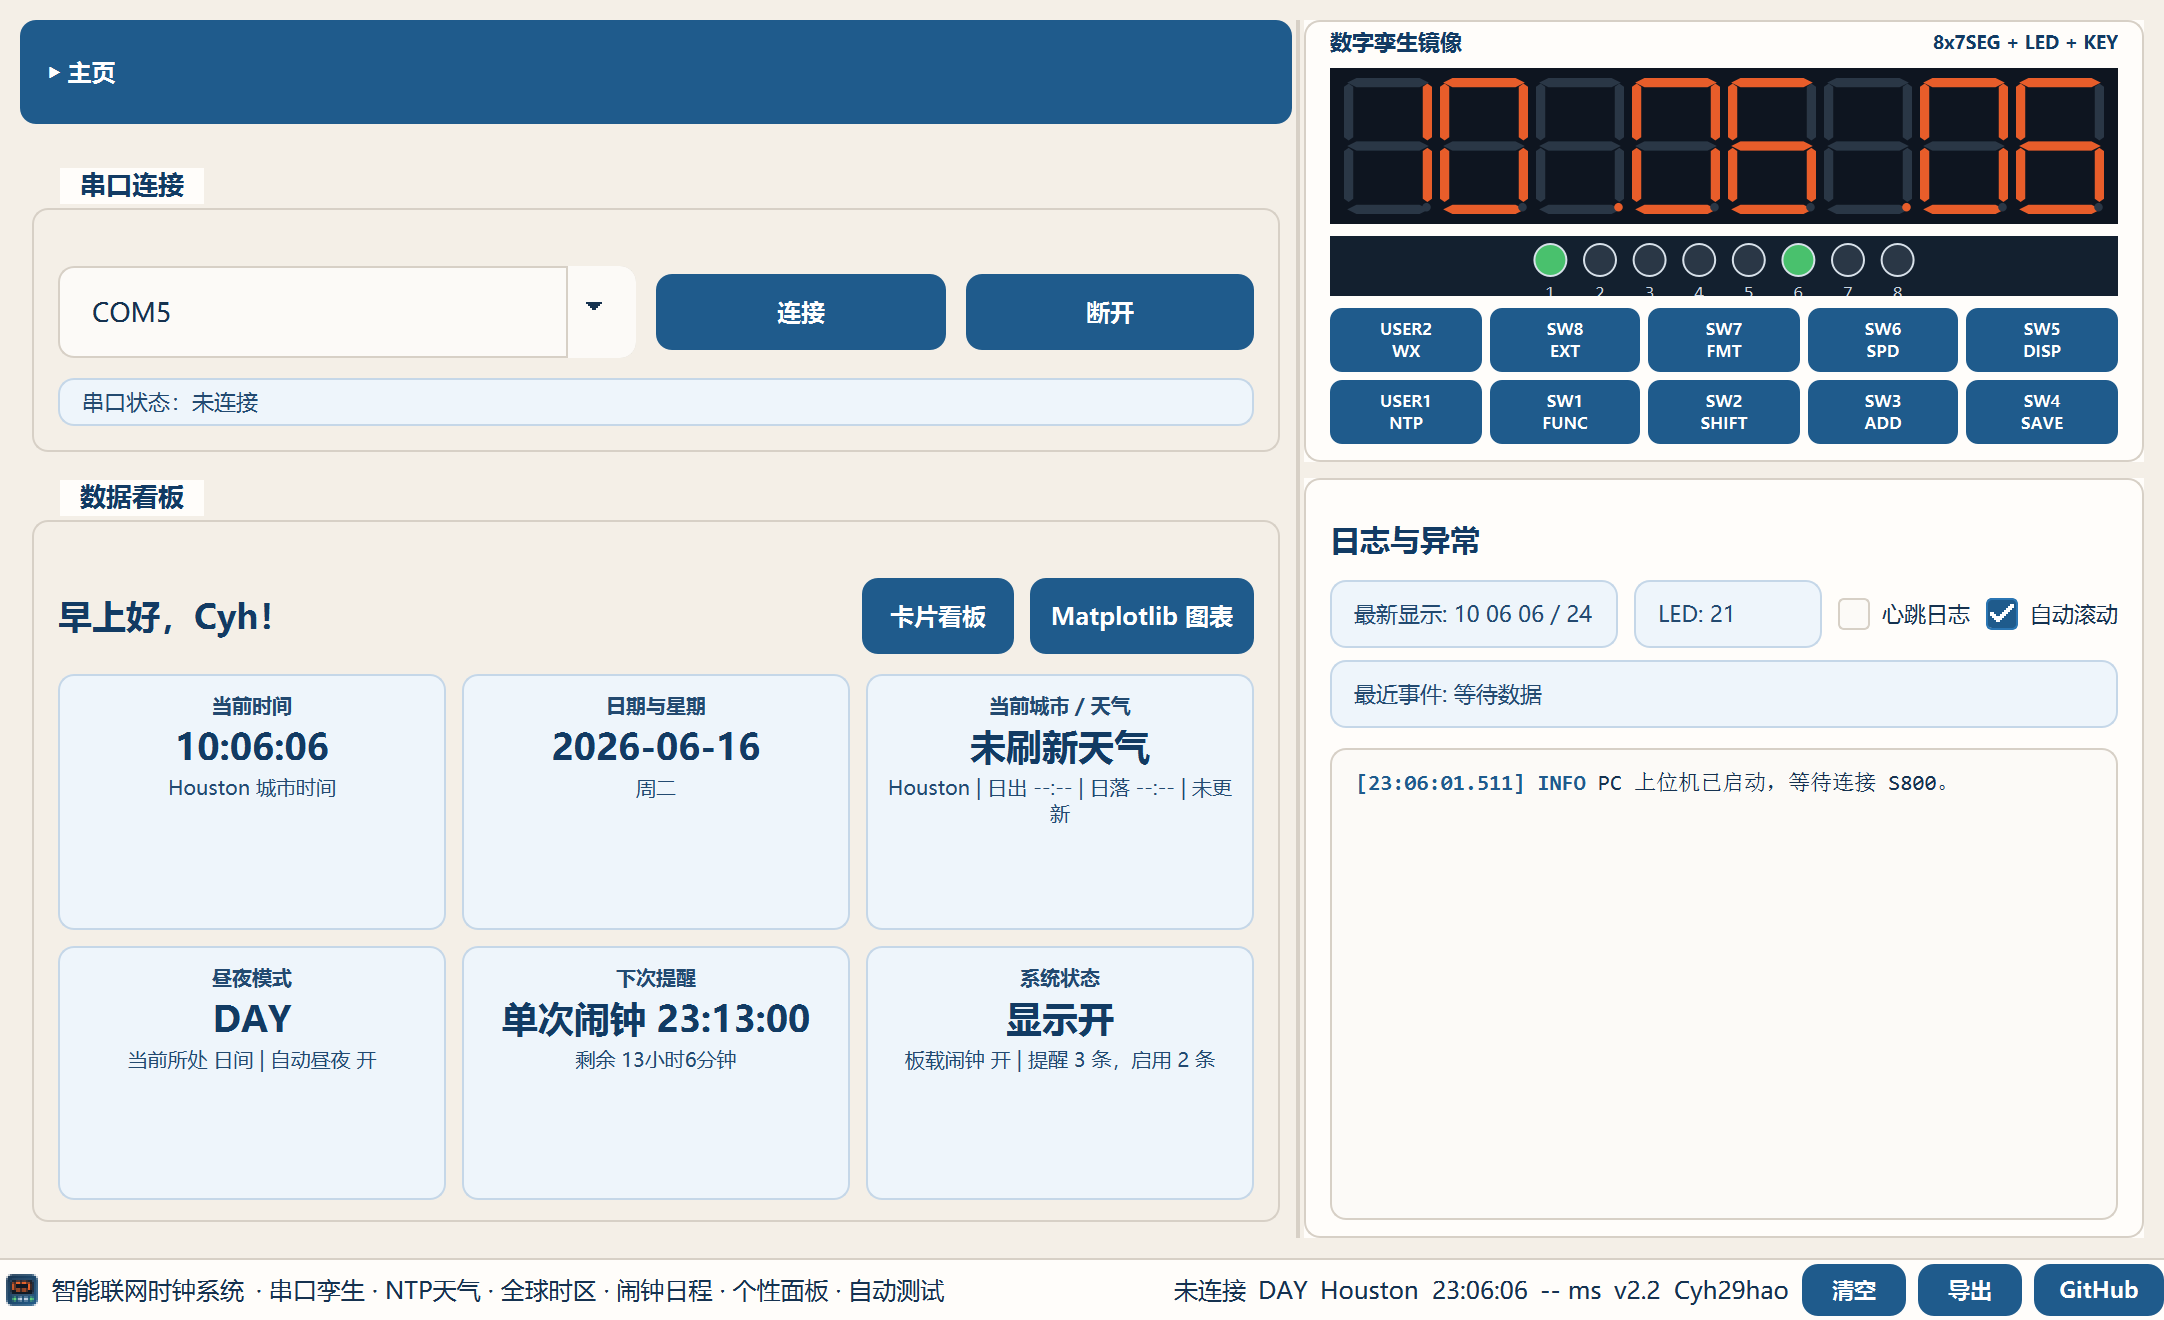
\includegraphics[width=0.96\linewidth]{pdf-home-dashboard.png}
\caption{PC 上位机主页：左侧为串口连接和数据看板，右侧为 8 位数码管、LED、按键和日志。}
\end{figure}

\subsection{最终交付物}
最终交付物不仅包含源码，还包含老师实际验收会用到的运行材料。MCU 端保留 Keil 工程、启动文件、Driverlib、\code{mcu/src/main.c} 和可烧录输出；PC 端保留 PyQt5 源码、UI 文件、依赖说明、启动脚本和打包 release；文档部分保留 README、验收对照、测试说明、截图、设计说明 PDF 和演示视频素材目录。这样的组织方式便于老师从源码、二进制运行、文档说明三个层面同时检查项目。

\section{课程要求与项目完成范围}
\subsection{要求来源与对照方式}
本项目依据课程大作业题目、MCU 与 PC 端开发要求、FAQ、testcmdV2.1 测试说明进行实现和自查。由于部分课程 PDF 是扫描/图片式文件，仓库中额外整理了 \code{docs/大作业要求逐条验收对照.md}，按原章节顺序转写核心要求，并把每一项对应到当前实现、演示方法和验证状态。本说明文档不替代源码和 README，但会把老师阅读时最需要知道的系统结构、功能覆盖和验证结果集中说明。

\begin{figure}[!htbp]
\centering
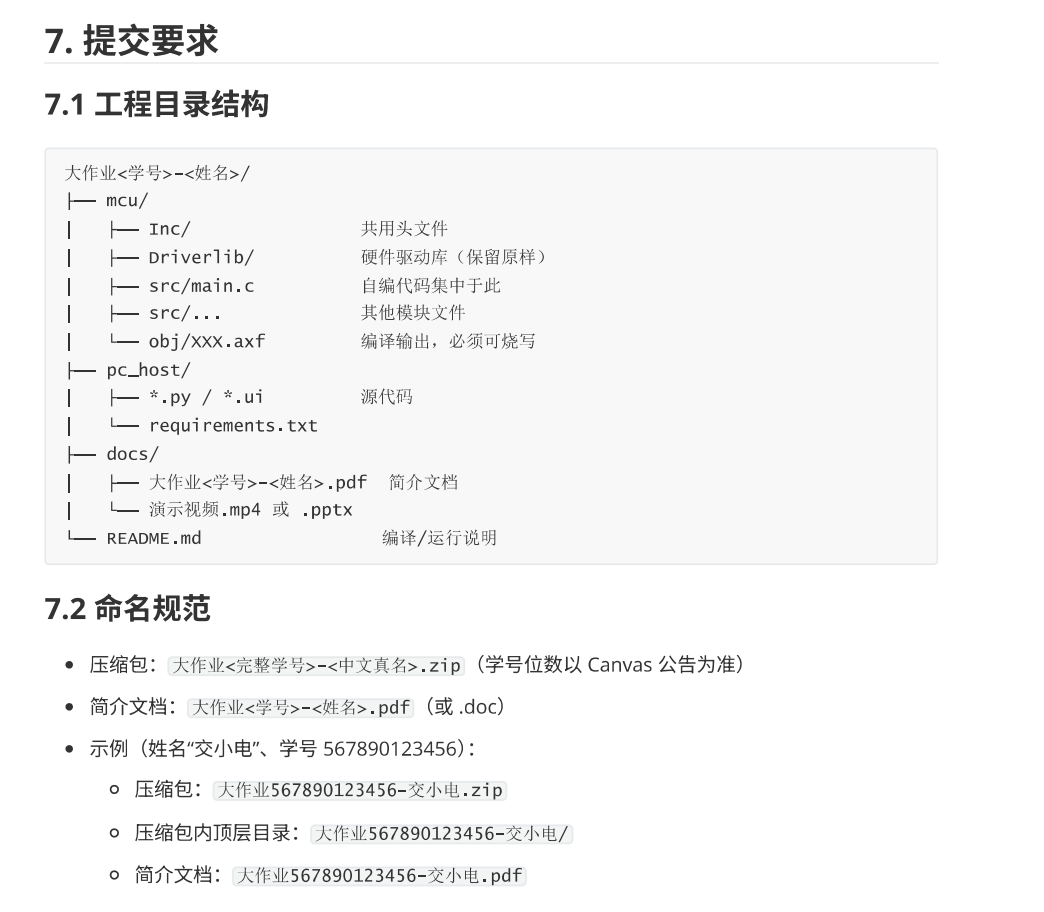
\includegraphics[width=0.72\linewidth]{course-submit-requirements.png}
\caption{课程提交要求截图：项目按 MCU、PC、文档、简介 PDF 和演示材料组织交付。}
\end{figure}

\subsection{基础要求覆盖}
S800 基础功能方面，项目实现了开机全亮/全灭、学号后八位、姓名拼音、版本号、默认时间显示、日期/星期/年份切换、LEFT/RIGHT 流水显示、两级速度、按键编辑、板载单次闹钟、LED 状态指示和蜂鸣反馈。串口协议方面，支持 \code{*SET}、\code{*GET}、\code{*PING}、\code{*EVT}、\code{OK} 和 \code{ERROR <reason>}；大小写、空格、缩写和行结束符均做了容错；非法参数、越界值、语法错误和超长帧会被明确拒绝。

PC 核心功能方面，项目实现了串口扫描、连接/断开、后台读、心跳延迟、状态栏、控制面板、协议日志、1:1 数字孪生、虚拟按键、错误高亮和日志导出。数字孪生完整包含 8 位七段数码管、8 位 LED、8 个矩阵按键和 USER1/USER2，并能根据板端 \code{*EVT:DISP}、\code{*EVT:LED}、\code{*EVT:KEY}、\code{*EVT:MODE} 更新。

\subsection{扩展和自主功能覆盖}
扩展功能 E1 到 E4 均已对应实现：E1 是 NTP 网络对时，E2 是天气获取和 USER2 天气短显，E3 是自动昼夜模式，E4 是 Matplotlib 数据可视化看板。自主功能部分以多日程/课程提醒系统为主，同时配合铃声预览、语音空文本规则、GitHub 版本管理、双向昼夜控制、自动测试脚本和高并发稳定性保护，形成比基础要求更完整的工程化体验。

\begin{table}[!htbp]
\centering
\caption{主要课程模块与项目实现对应}
\begin{tabularx}{\linewidth}{>{\bfseries}p{0.22\linewidth}X>{\centering\arraybackslash}p{0.13\linewidth}}
\toprule
模块 & 当前实现 & 状态\\
\midrule
S800 基础时钟 & 开机动画、时间日期、星期/年份、滚动、按键编辑、闹钟、LED、蜂鸣、离线运行。 & 完成\\
串口协议 & ASCII 帧、SET/GET/PING/EVT、ERROR 分类、RIGHT 格式、小数点跟随、老师 testcmd 语法。 & 完成\\
PC 上位机 & 串口管理、控制面板、日志、数字孪生、虚拟按键、异常提示、打包 exe。 & 完成\\
扩展功能 & NTP、天气、自动昼夜、Matplotlib 今日时间轴/提醒分布/系统状态/日志统计。 & 完成\\
自主设计 & 多日程提醒、铃声预览、全球时区、自动测试、高并发防卡死、GitHub 管理。 & 完成\\
提交材料 & README、验收对照、测试记录、release、设计说明 PDF、演示素材目录。 & 已整理\\
\bottomrule
\end{tabularx}
\end{table}

\section{总体架构：硬件端、PC 端与协议协同}
\subsection{架构分工}
系统采用“实时硬件逻辑在 MCU，复杂交互和网络逻辑在 PC”的分工。MCU 负责 1 ms 时基、七段数码管扫描、按键防抖、日期时间推进、闹钟、蜂鸣、LED 和串口协议；PC 负责界面布局、串口收发、日志、网络对时、天气、全球时区、日程、图表和自动测试。这样可以避免在 MCU 上堆叠过多网络和界面逻辑，同时保证 PC 的网络慢、天气失败或图表加载不会破坏板端基本走时。

\begin{table}[H]
\centering
\caption{系统总体架构与数据流}
\begin{tabularx}{\linewidth}{>{\bfseries}p{0.22\linewidth}p{0.23\linewidth}X}
\toprule
层次 & 主要内容 & 数据流说明\\
\midrule
PC 上位机界面 & 页面、日志、数字孪生、图表 & 用户操作形成串口命令；板端事件刷新界面、状态栏和镜像。\\
PC 扩展服务 & NTP、天气、时区、日程、测试 & 后台任务产生时间、天气、提醒和测试结果，再交给 UI 层排队下发或展示。\\
USB 虚拟串口 & 115200 8N1 ASCII & PC 发送 SET/GET/PING；MCU 返回 OK/ERROR/PONG/EVT。\\
TM4C1294 主程序 & 时钟、显示、状态机、协议解析 & 非阻塞主循环处理硬件和协议，主动上报显示、LED、按键和闹钟事件。\\
S800 外设 & 七段数码管、LED、按键、蜂鸣 & MCU 直接扫描、读取和驱动，保证离线时钟仍能独立运行。\\
\bottomrule
\end{tabularx}
\end{table}

\subsection{数据流与控制流}
控制流从 PC 到 MCU：用户点击界面按钮、协议台发送命令、自动测试脚本执行步骤，最终都会形成 \code{*SET}、\code{*GET} 或 \code{*PING} 命令写入串口。MCU 解析命令后立即返回 \code{OK}、查询结果或 \code{ERROR <reason>}，并在需要时改变板端显示、LED、闹钟或模式。

数据流从 MCU 到 PC：板端显示变化、LED 变化、物理按键、闹钟开始/停止、编辑保存和模式切换都会以 \code{*EVT:*} 主动上报。PC 收到事件后刷新日志、状态栏、数字孪生和相关表单。这样 PC 不需要盲猜板端状态，而是以板端回传为真实依据。

\subsection{数字孪生的数据源优先级}
数字孪生镜像的数据源优先级是项目稳定性的关键。串口已连接并收到板端真实显示帧时，镜像无条件以 \code{*EVT:DISP} 和 \code{*EVT:LED} 为准；串口已连接但短时间未收到新帧时，镜像保留最后一帧或显示等待状态；只有未连接串口或明确离线模拟时，PC 才使用本地影子状态生成显示。这个规则保证 RESET 开机画面、物理按键和板端真实显示不会被 PC 的天气刷新、NTP、图表或测试提示覆盖。

\section{S800/TM4C1294 板端设计}
\subsection{硬件资源与程序职责}
板端主程序位于 \code{mcu/src/main.c}。程序启动后初始化系统时钟、SysTick、I2C、UART、LED、按键和蜂鸣器相关资源，然后进入非阻塞主循环。主循环持续处理 UART 输入、按键扫描、显示刷新、蜂鸣节拍、闹钟检查和临时显示超时，避免长时间阻塞导致串口丢字节或显示停顿。

\begin{table}[!htbp]
\centering
\caption{S800 板端硬件资源与实现内容}
\begin{tabularx}{\linewidth}{>{\bfseries}p{0.19\linewidth}X}
\toprule
硬件资源 & 实现内容\\
\midrule
8 位七段数码管 & 时间、日期、星期、年份、开机动画、编辑内容、滚动消息、天气短显、板端标签。\\
8 位 LED & D1 心跳、D2 闹钟、D3 编辑、D4 串口 RX、D5 串口 TX、D6 夜间、D7 RIGHT、D8 手动覆盖。\\
SW1--SW8 & FUNC、SHIFT、ADD、SAVE、DISP、SPEED、FORMAT、EXT。\\
USER1/USER2 & USER1 短按触发 PC 对时、长按切换 DAY/NIGHT；USER2 用于天气短显。\\
蜂鸣器 & 闹钟响铃、日程提醒、远程蜂鸣、不同铃声节奏。\\
UART0 & ASCII 串口协议，接收 PC 命令并上报事件。\\
EEPROM/备份逻辑 & 保存最近时间，RESET 后尽量从最近时间恢复，不直接回到 00:00:00。\\
\bottomrule
\end{tabularx}
\end{table}

\subsection{时基、日期和显示逻辑}
程序使用 1 ms SysTick 作为基础时基。中断本身只做轻量计数，真正的显示、按键、蜂鸣和串口处理在主循环中按节拍推进。时间推进每 1000 ms 执行一次，日期逻辑包含闰年、月末进位和 23:59:59 到 00:00:00 的转换。默认时间页显示时分秒，DISP 按键循环切换时间、日期、星期和年份。NIGHT 模式下普通时间页显示时分，减少夜间干扰；但进入 FUNC 时间编辑页时仍显示完整时分秒，方便准确编辑。

七段数码管一次只能显示 8 位，因此长文本通过滚动状态机显示。滚动消息、星期、日期长文本和日程板端标签会在端点停顿，至少往返碰到一次左端；最后一帧额外停约 2 秒再恢复时钟。PC 和 MCU 两端都会拒绝或转义不支持字符，真实下划线显示为七段码底段，避免非法字符导致状态机卡死。

\noindent\textbf{显示事件和点阵同步的串口形式示例}
\begin{verbatim}
*EVT:DISP 12_30_45 24
*EVT:LED 21
*SET:MSG A_B_TEST
\end{verbatim}

\subsection{按键、防抖与编辑状态机}
板端按键采用周期扫描和稳定计数进行防抖。FUNC、SHIFT、ADD、SAVE 构成编辑状态机：FUNC 在日期、时间、闹钟编辑页之间切换，SHIFT 选择字段，ADD 修改字段，SAVE 或 FUNC 长按保存退出，超时无操作会自动退出且不保存。EXT 用于退出临时显示、编辑态或关闭板载单次闹钟，避免用户在连续操作后停留在无法回到默认时间页的状态。

USER1、USER2、FUNC、DISP 等容易造成状态叠加的按键做了冷却和长按判定。USER1 短按触发 PC 对时，长按切换昼夜模式；USER2 定义为天气短显；DISP 长按可切换显示开关，短按只切换显示页。串口模拟按键和 PC 虚拟按键也尽量采用相同语义，减少物理操作和软件操作的差异。

\subsection{闹钟、日程提醒与蜂鸣}
板载单次闹钟保存在 MCU 状态中，到点后启动蜂鸣器和 LED 提示，FUNC 可以立即停止响铃，程序也会限制最长响铃时间。PC 日程提醒不是简单在 PC 弹一行日志，而是会把板端标签、滚动短显和铃声命令发送到 MCU，日志记录实际触发的铃声名称。这样课程提醒、会议提醒、提交检查等 PC 管理事项也能在实物板上产生可观察反馈。

\subsection{LED 位义}
8 位 LED 在本项目中不是装饰，而是系统状态的一部分。D1 表示运行心跳，D2 表示板载单次闹钟启用或响铃闪烁，D3 表示编辑状态，D4/D5 表示串口 RX/TX 活动，D6 表示夜间模式，D7 表示 RIGHT 显示方向，D8 表示手动 LED 覆盖。天气短显期间，LED 会按天气掩码短时覆盖，短显结束后恢复系统状态位。PC 调试页中的 \code{*SET:LED XX} 可手动设置掩码，用于验收逐位点亮和调试。

\section{PC 上位机设计}
\subsection{界面整体组织}
PC 上位机是本项目产品化程度最高的部分。它不是把串口命令简单堆在一起，而是按实际使用场景组织页面：主页负责总览，系统设置负责全局配置，闹钟与日程管理负责提醒业务，调试与测试负责协议和验收。右侧数字孪生区域始终可见，底部状态栏持续显示系统功能和连接状态。布局遵循左侧主功能区、右侧展示区、底部状态栏三块结构，避免右侧覆盖左侧或日志压住按键。

\begin{figure}[!htbp]
\centering
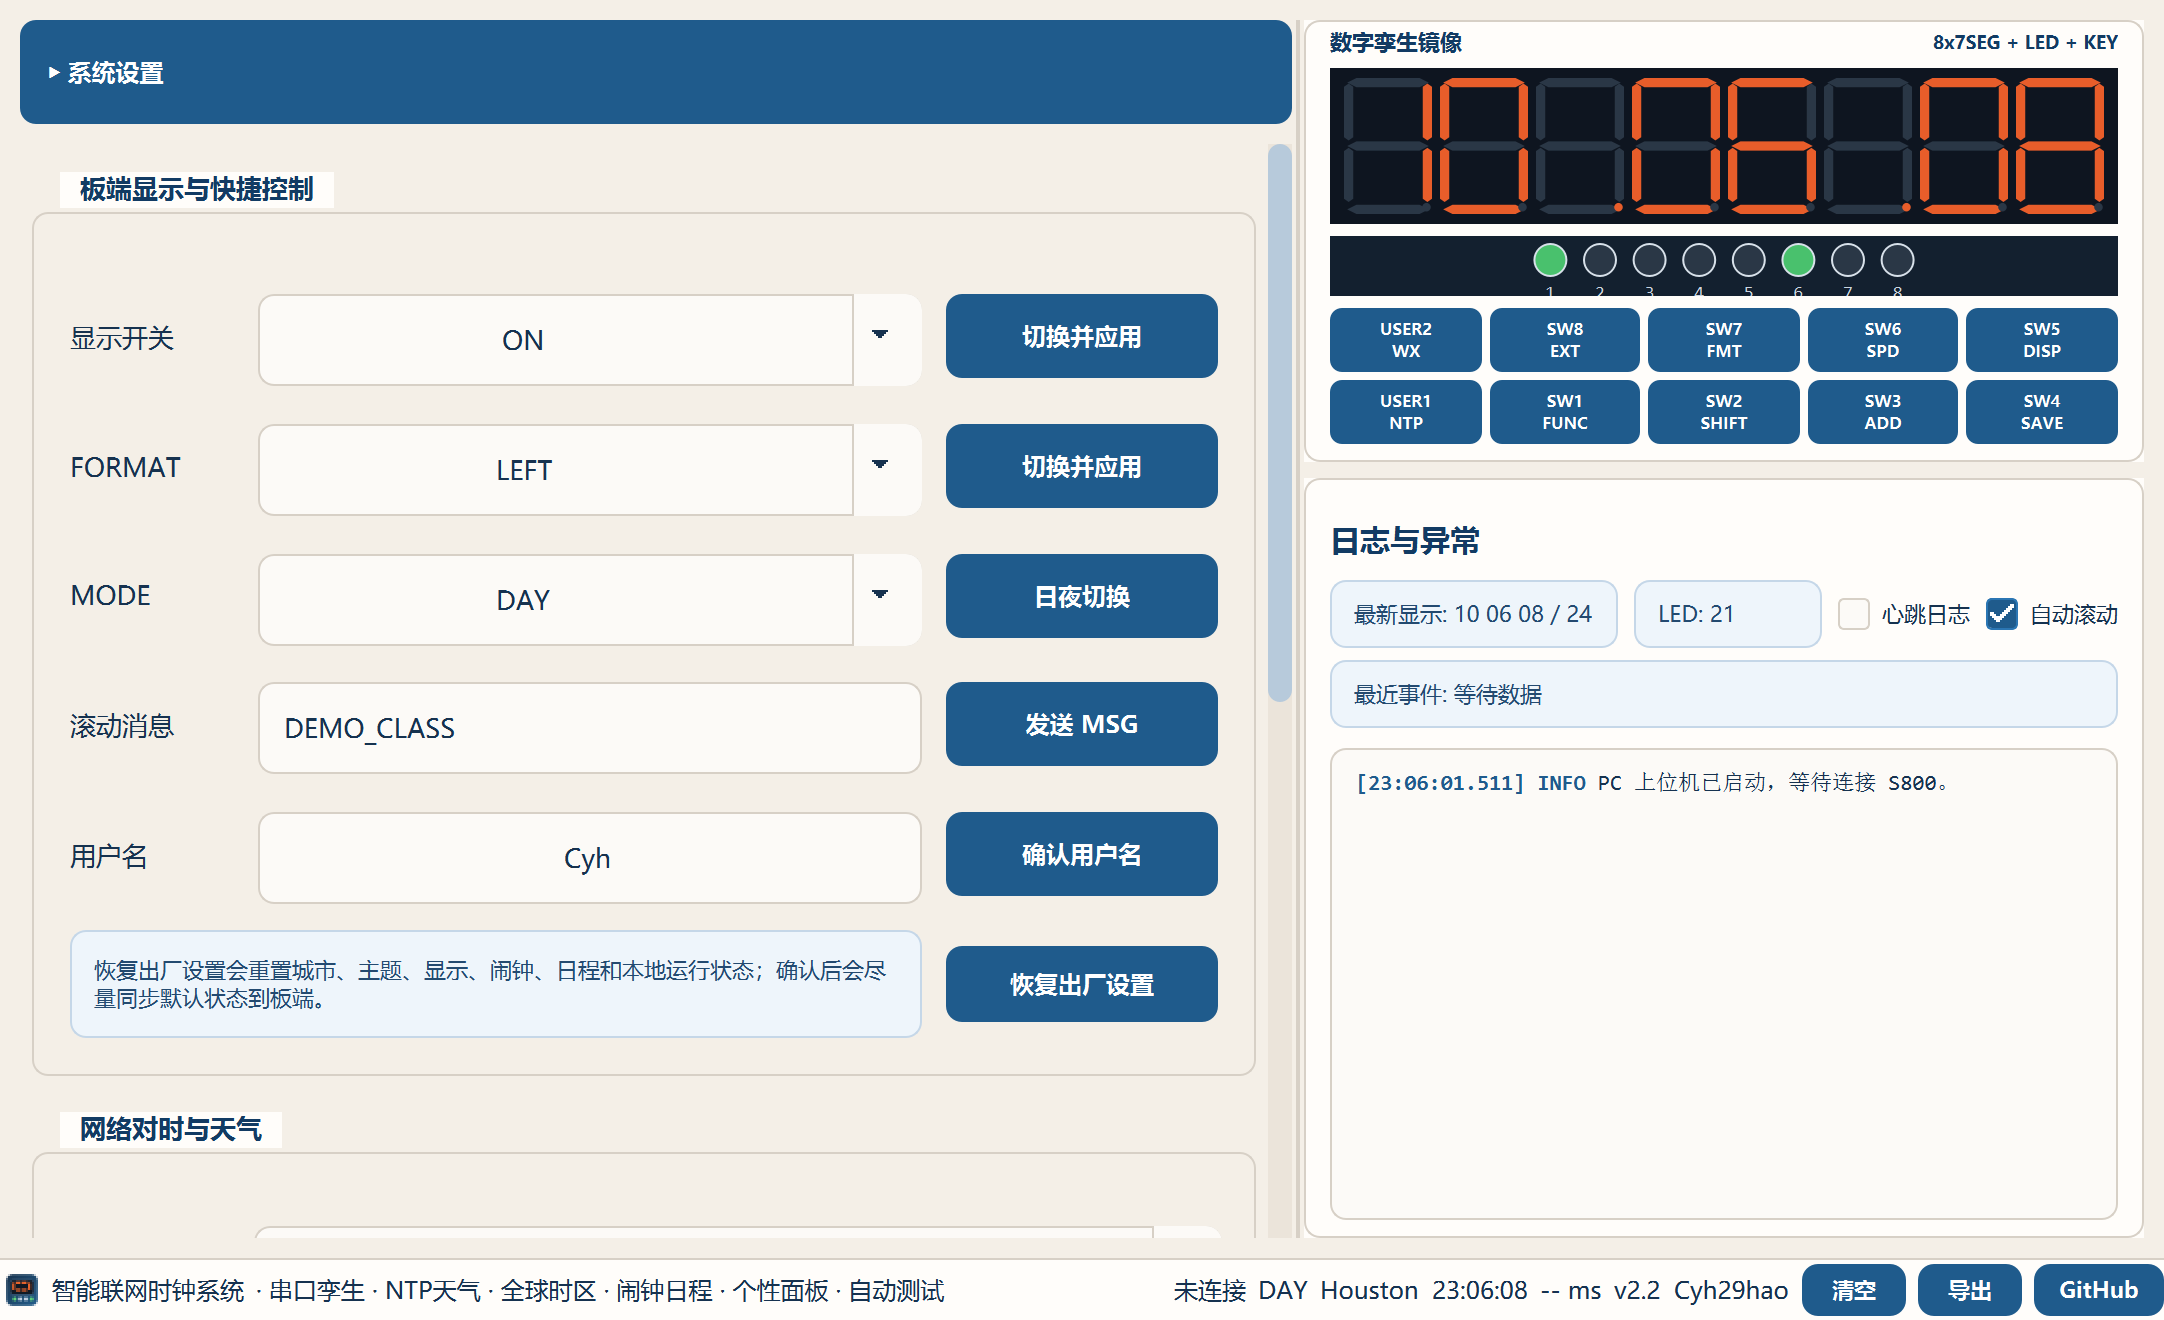
\includegraphics[width=0.96\linewidth]{pdf-system-settings.png}
\caption{系统设置页：全局显示、DAY/NIGHT、城市/时区、自动昼夜、恢复出厂设置集中管理。}
\end{figure}

\subsection{主页卡片看板与 Matplotlib 图表看板}
主页默认展示卡片式数据看板，包括当前时间、日期星期、城市天气、昼夜模式、下一次提醒、系统状态和问候语。卡片看板适合老师快速了解系统当前状态，也适合没有串口时离线演示。

为了完成扩展功能 E4，主页新增 Matplotlib 图表看板，与卡片看板通过切换按钮无缝切换。图表提供四类过滤视图：今日时间轴、提醒分布、系统状态、过去 24 小时日志统计。系统状态图使用“0/1”“1/5”“正常/开”等直接状态表达，不使用容易误解的百分比。日志统计从本地事件日志中按板端显示、NTP/天气、闹钟日程、昼夜模式、自动测试、系统设置和错误警告分类。

\begin{figure}[!htbp]
\centering
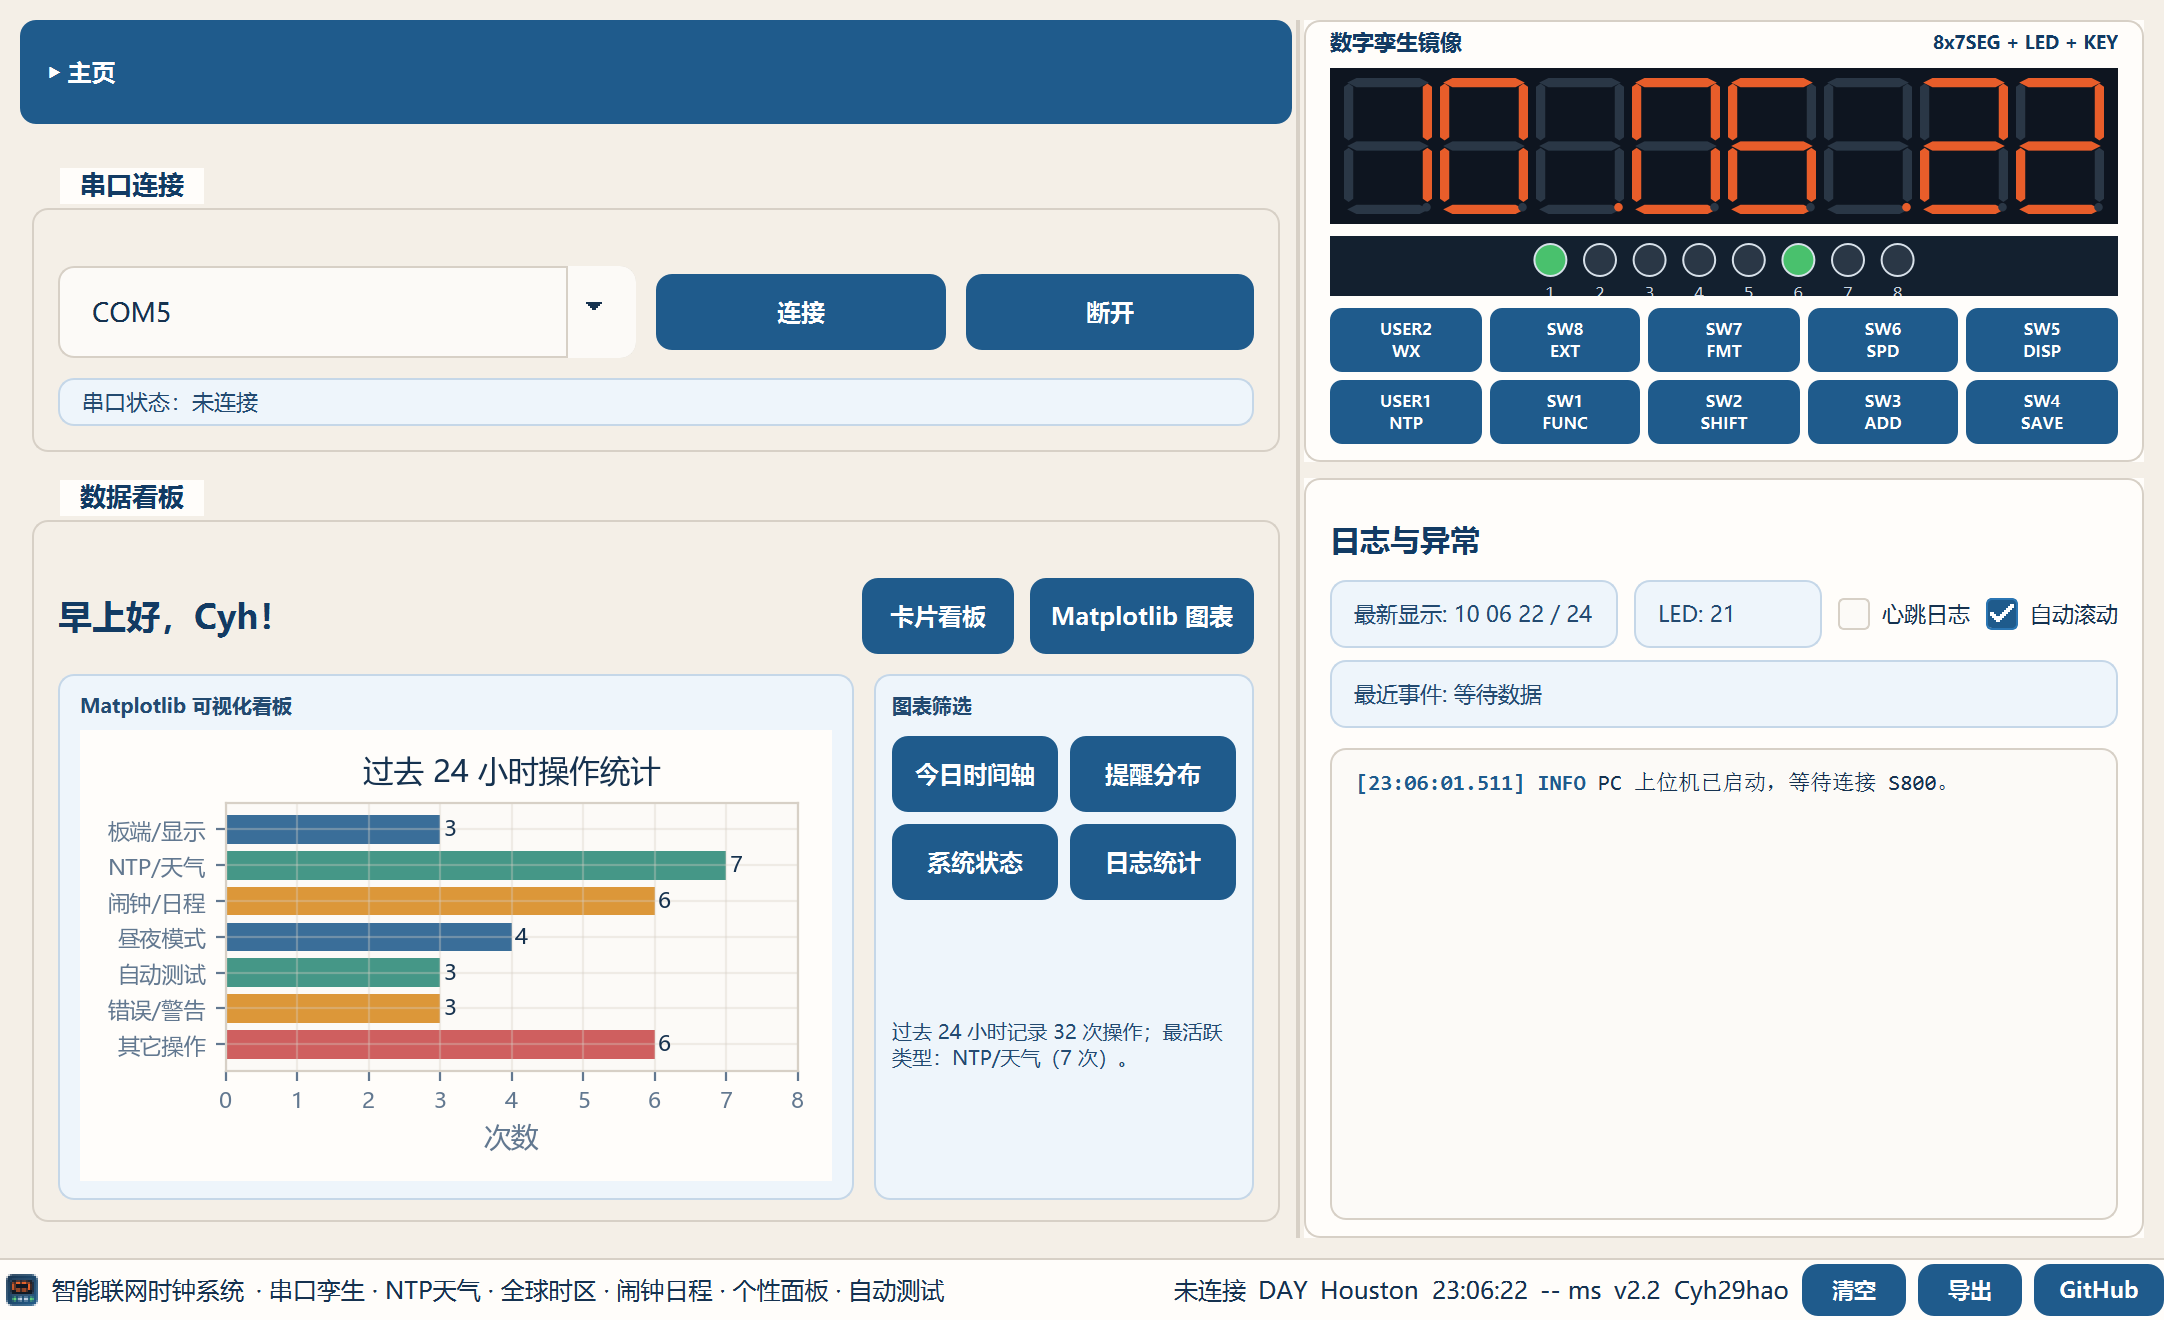
\includegraphics[width=0.96\linewidth]{pdf-matplotlib-log-stats.png}
\caption{Matplotlib 日志统计视图：从过去 24 小时事件记录中展示系统操作分布。}
\end{figure}

\subsection{数字孪生镜像与交互细节}
右侧数字孪生镜像包含 8 位七段数码管、8 位 LED、SW1--SW8 和 USER1/USER2。每个按键都有鼠标悬停说明，例如 DISP 用于时间、日期、星期、年份切换，USER1 长按切换 DAY/NIGHT，USER2 显示天气短显。虚拟按键支持短按和约 0.8 秒长按，使 PC 操作和实物按键语义更一致。

数字孪生还承担“解释硬件”的作用。老师看到右侧镜像时，不需要猜某个 LED 或按键代表什么，界面提示和调试页说明会给出 D1-D8 位义、LED 掩码用途和按键功能。串口已连接时，它优先显示板端真实帧；未连接时，它又能作为离线模拟展示工具。

\subsection{网络对时、全球时区与天气}
网络对时和天气被设计成一个可理解的多步骤流程。用户输入城市或国家后，程序先定位城市或国家首都，获取经纬度、国家信息和 IANA 时区；然后执行 NTP 或 HTTP Date 对时；最后拉取天气、日出日落和 UTC offset。日志会依次提示“正在定位”“时区已获取”“正在拉天气”“天气已刷新”“开始 NTP 对时”等阶段，让用户知道等待发生在什么环节。

全球时区主要使用 Open-Meteo Geocoding 和 Open-Meteo Forecast；失败时尝试 Nominatim 地理编码和 wttr.in 天气兜底。Houston、Chicago、London、Tokyo、Paris、New Delhi、Sydney 以及中国、美国、日本、澳大利亚等常见城市/国家有内置预设，网络不稳时仍可获得基本时区和坐标。PC 以获取到的城市时间作为基准，再用单调时钟本地推进，避免 UI 定时器误差造成走时偏快。

\subsection{日程管理与提醒体验}
日程管理支持单次日期和每周重复，包含标题、板端标签、触发时间、铃声、语音文本和启用状态。默认新建时间设置为当前小时、当前分钟加 1，方便现场测试。表格空白区域可以取消当前选中项，避免用户选中旧日程后不好回到新建状态。铃声选择旁有预览按钮，语音播报按闹钟和日程分别控制，文本为空时默认不播报。

\begin{figure}[!htbp]
\centering
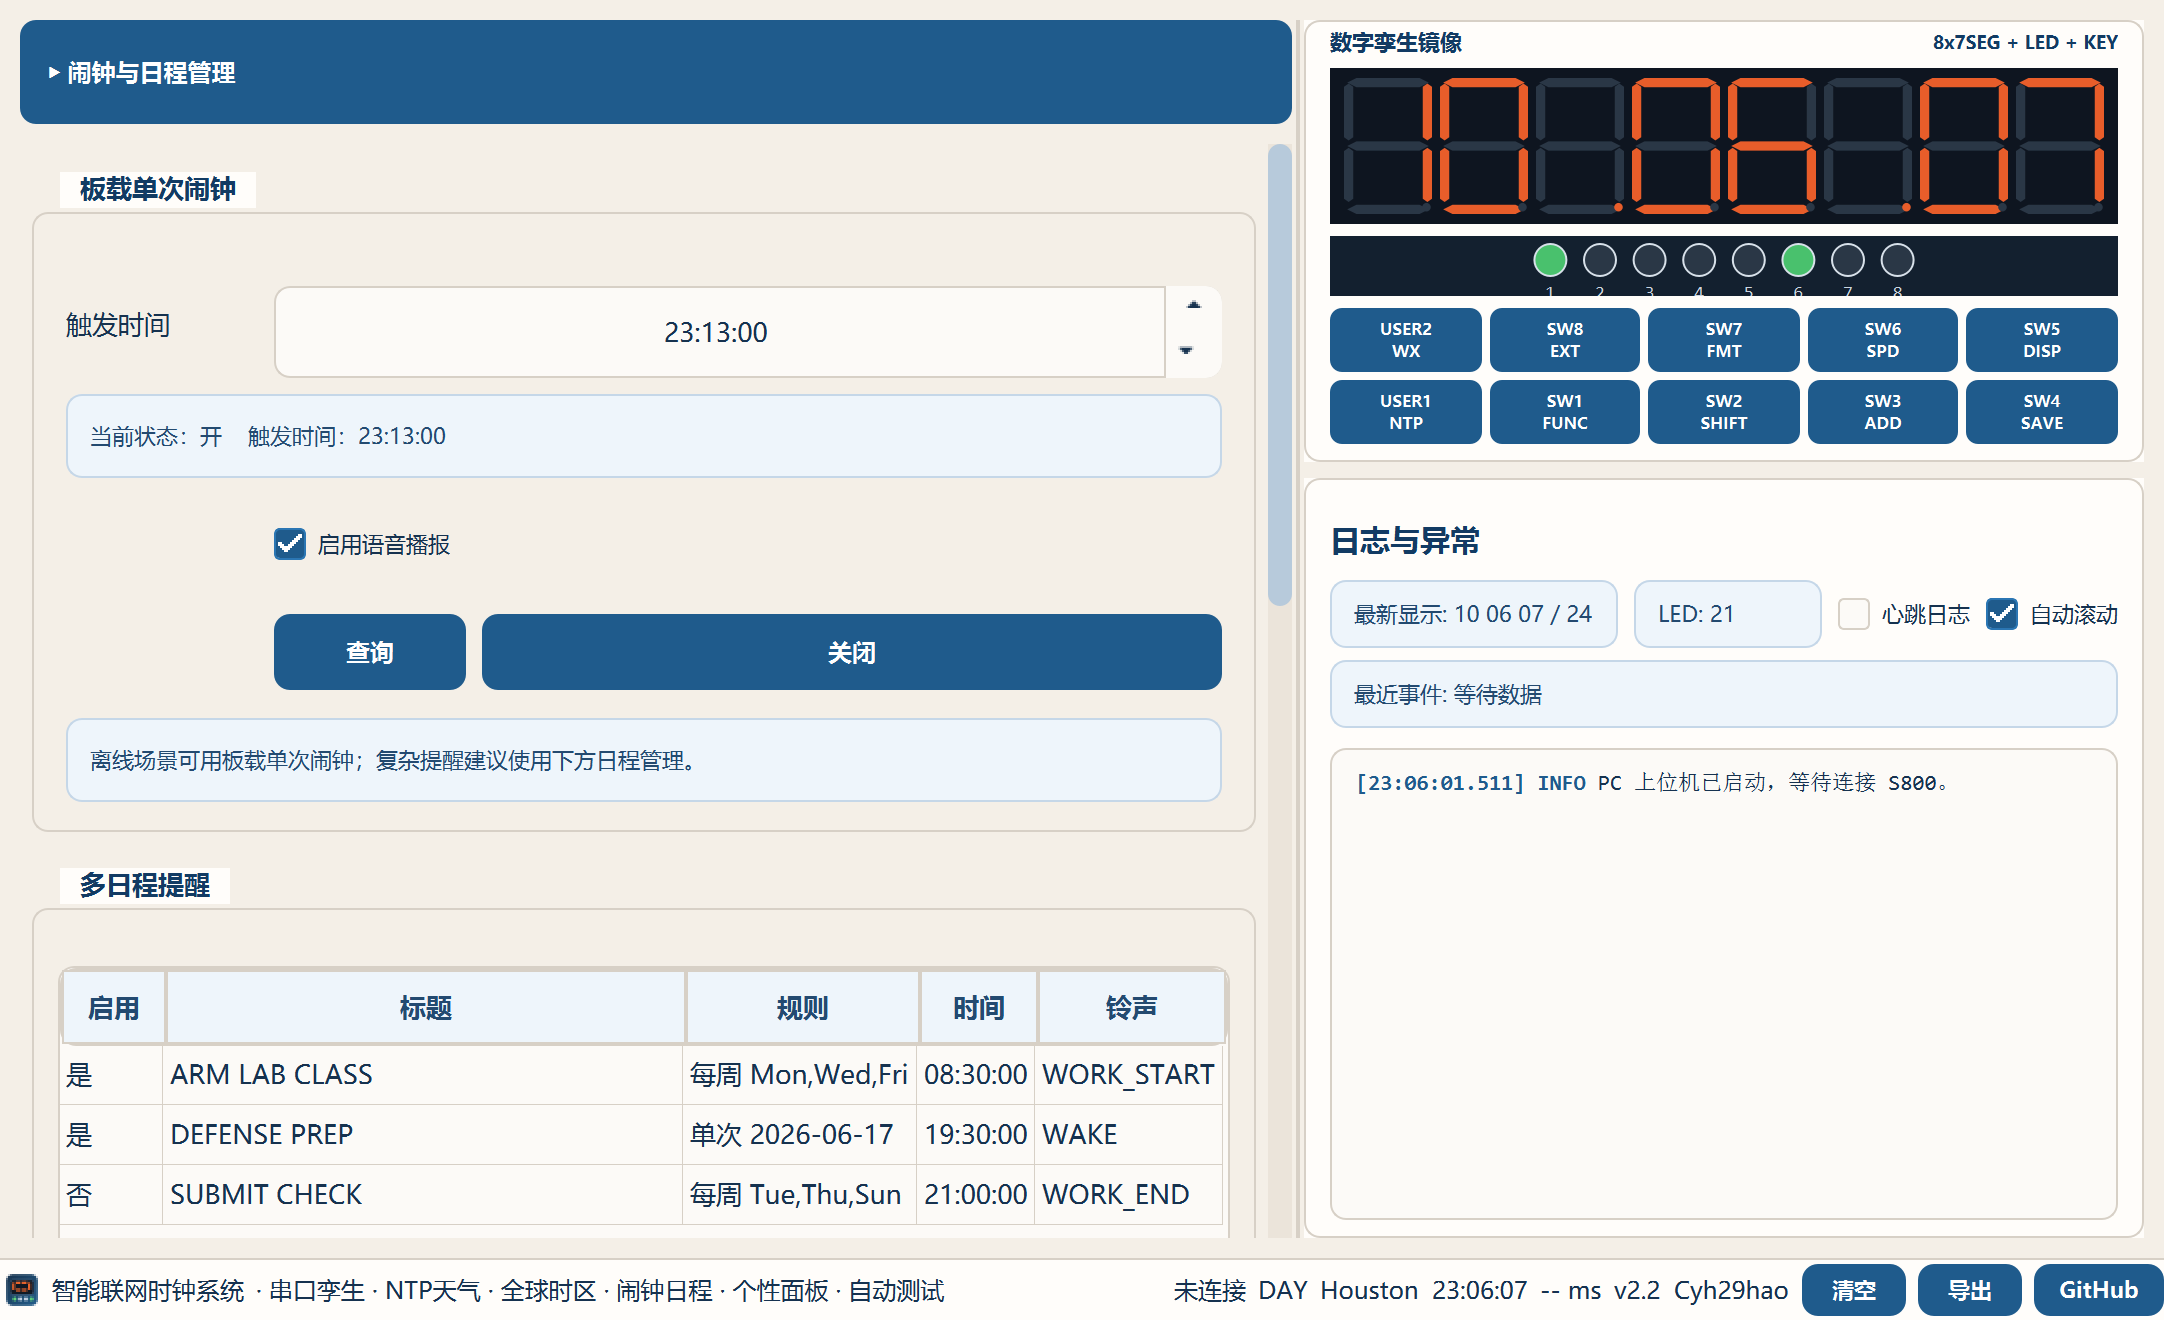
\includegraphics[width=0.96\linewidth]{pdf-schedule-demo.png}
\caption{闹钟与日程管理页：示例日程展示了每周实验课、演示准备和提交检查等使用场景。}
\end{figure}

\subsection{调试与测试页面}
调试与测试页面把课程验收中最常用的人工操作集中到一个入口。时间与写入区区分手动编辑写入和 NTP 自动对时写入；板端硬件测试区保留蜂鸣和 LED 掩码输入；协议测试台下拉框覆盖所有主要命令模板，随机混合大小写和缩写当前指令都作用于当前命令；错误格式测试覆盖 \code{ERROR LEN}、\code{ERROR SYNTAX}、\code{ERROR PARAM}、\code{ERROR RANGE}。快速联合测试和全面联合测试带步骤进度、失败即停、中止按钮、测试后设置恢复和页脚“测试中”提示。

\begin{figure}[!htbp]
\centering
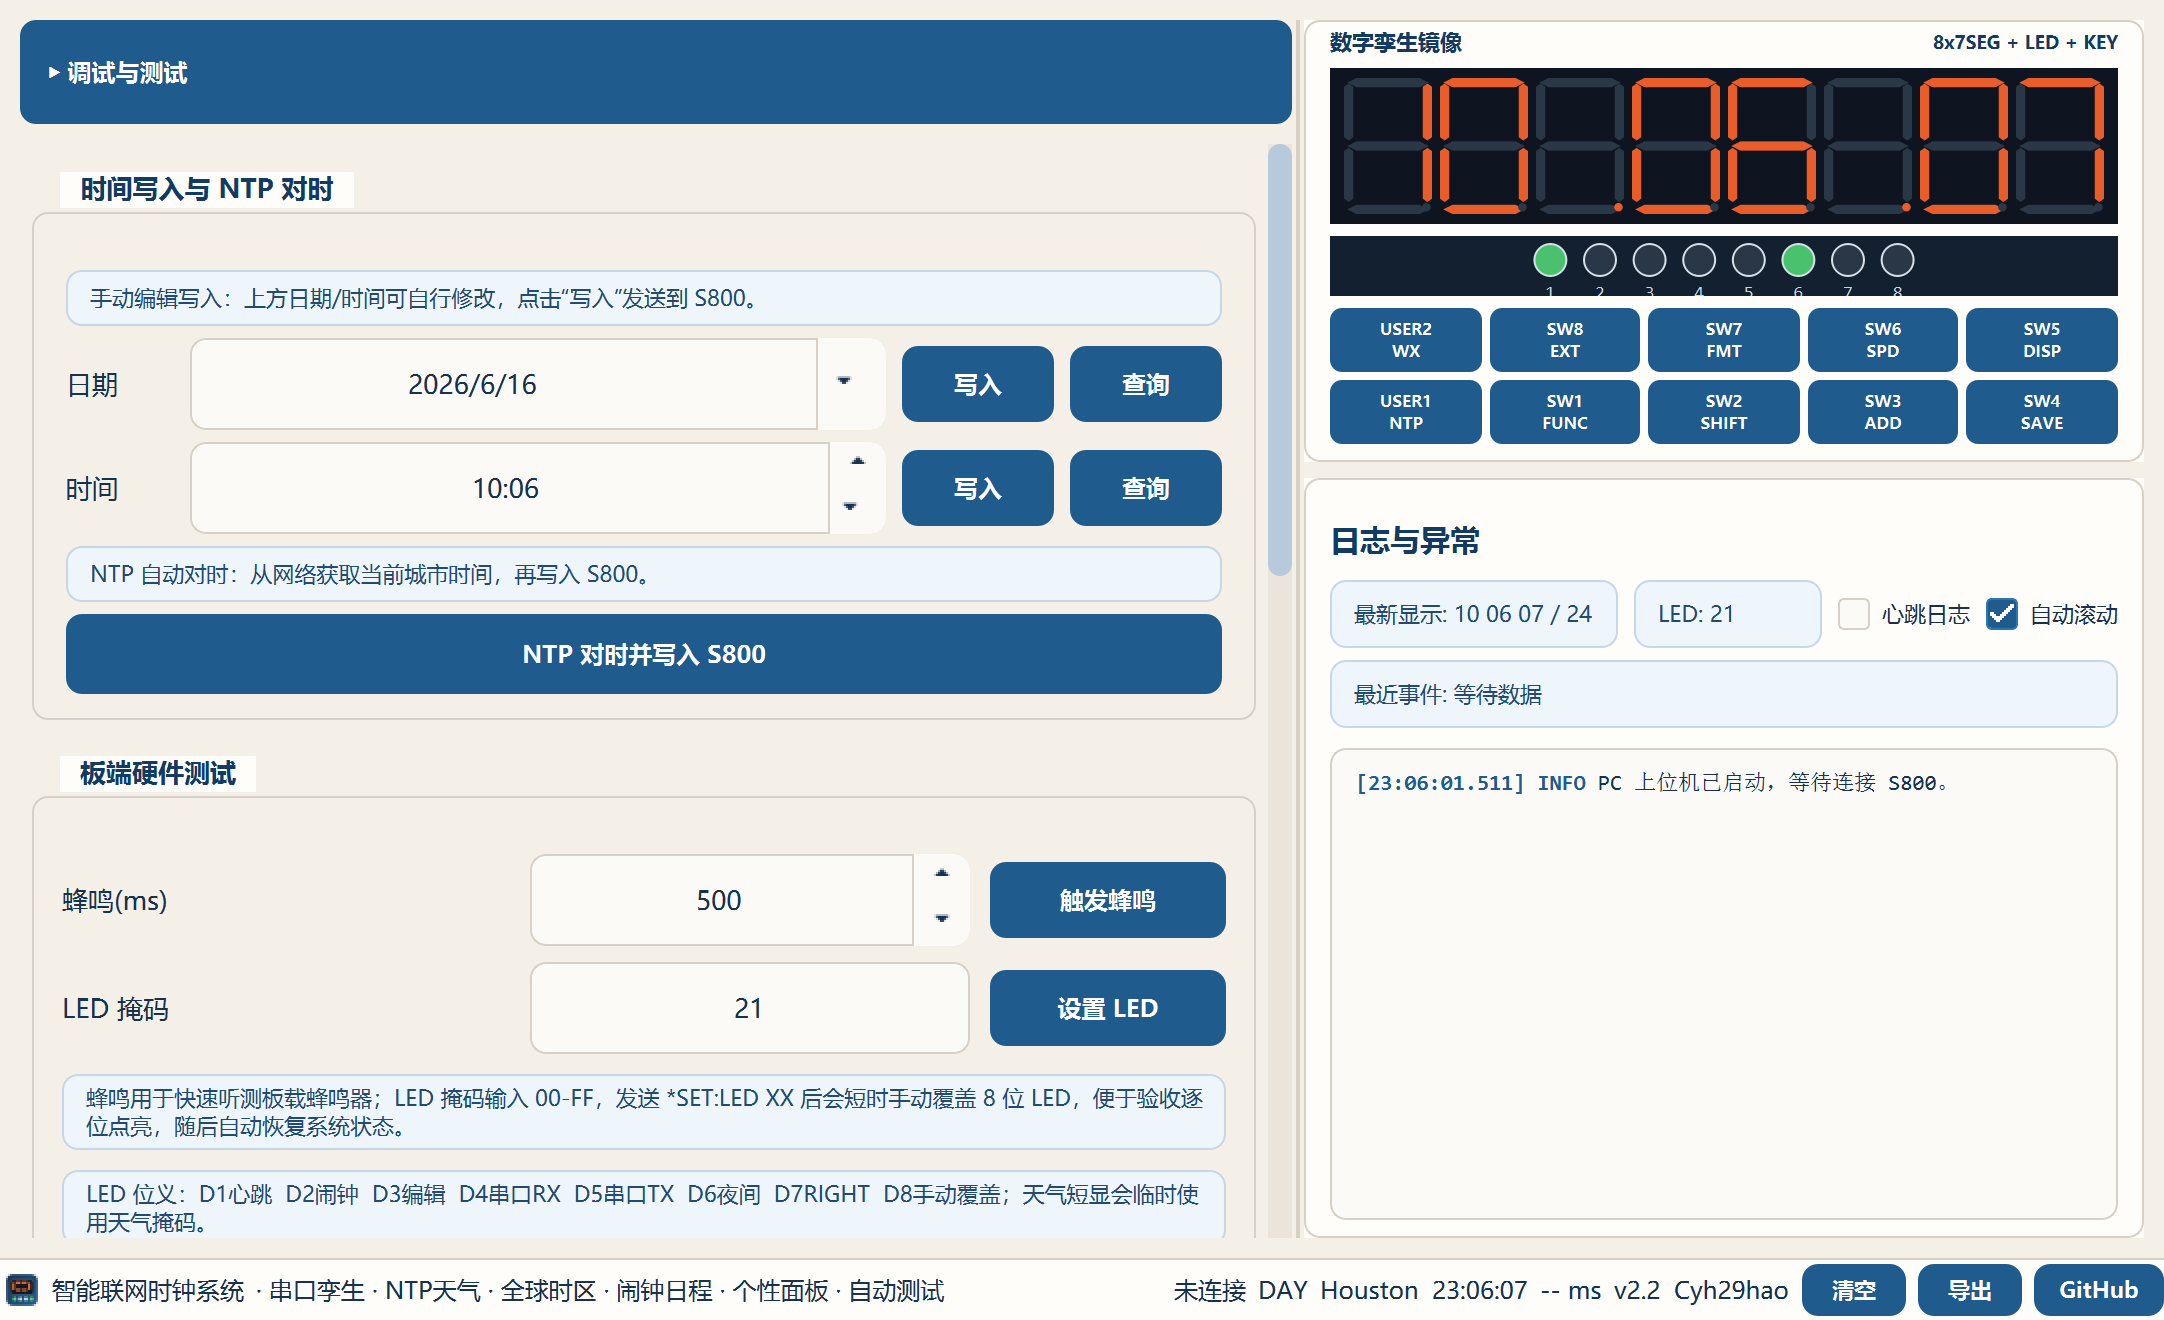
\includegraphics[width=0.96\linewidth]{pdf-debug-test.png}
\caption{调试与测试页：手动协议、硬件测试和自动化测试共用一个清晰入口。}
\end{figure}

\section{串口协议与双向同步}
\subsection{协议基本格式}
串口协议采用 115200、8N1、ASCII 文本帧，无硬件流控。命令以星号开头，行结束符兼容回车、换行和二者组合。单帧长度有限制，超长会返回 \code{ERROR LEN}。命令大小写不敏感，多余空格可容忍，部分字段支持明确缩写；但错误缩写、缺少参数和越界参数不会被放行，而是返回对应 ERROR。

\noindent\textbf{典型串口会话示例}
\begin{verbatim}
PC  -> *PING
MCU <- *PONG 36
PC  -> *SET:DATE YEAR MONTH DATE 2026 06 16
MCU <- OK
PC  -> *SET:TIME HOUR MIN SEC 19 30 00
MCU <- OK
MCU <- *EVT:DISP 19_30_00 24
MCU <- *EVT:LED 01
\end{verbatim}

\subsection{主要命令与事件}
\begin{longtable}{>{\ttfamily}p{0.27\linewidth}p{0.67\linewidth}}
\caption{主要串口命令和事件说明}\\
\toprule
命令/事件 & 作用\\
\midrule
\endfirsthead
\toprule
命令/事件 & 作用\\
\midrule
\endhead
*RST & 复位运行状态，恢复 DISPLAY=ON、FORMAT=LEFT 等默认设置。PC 端会合并生命周期 NTP，避免重复对时。\\
*PING & 板端返回 *PONG <uptime>，用于连通性和延迟检查。\\
*SET:DATE / *SET:TIME & 写入日期和时间，支持老师 testcmd 使用的字段组 + 数值组语法，也兼容旧交替参数语法。\\
*SET:ALARM / *GET:ALARM & 设置、关闭和查询板载单次闹钟。\\
*SET:DISPLAY / *SET:FORMAT / *SET:MODE & 控制显示开关、LEFT/RIGHT 显示方向和 DAY/NIGHT 模式。\\
*SET:MSG / *SET:WEATHER & 发送滚动消息和天气短显 token。\\
*SET:BEEP / *SET:LED / *SET:KEY & 远程蜂鸣、LED 掩码覆盖、模拟按键。\\
*EVT:DISP / *EVT:LED & 板端主动上报数码管显示帧和 LED 状态，是数字孪生的主要数据源。\\
*EVT:KEY / *EVT:MODE & 上报物理按键和昼夜模式变化，用于 PC 端同步主题和状态。\\
*EVT:ALARM / *EVT:EDIT & 上报闹钟开始/停止和板端本地编辑保存。\\
\bottomrule
\end{longtable}

\subsection{PC 与板端的双向控制}
PC 和板端不是单向主从。PC 可以通过按钮、协议台和自动测试控制板端；板端也可以通过物理按键影响 PC。典型例子是昼夜模式：PC 按钮或自动昼夜会下发 \code{*SET:MODE DAY/NIGHT}，板端 USER1 长按也会产生 \code{*EVT:MODE DAY/NIGHT} 并使 PC 主题跟随变化。再如 USER1 短按，板端只发事件，PC 收到后执行 NTP 对时并写回板端。

\subsection{错误处理和稳定性保护}
串口错误格式统一为 \code{ERROR <reason>}。协议台和自动测试会专门发送错误模板，验证非法命令不会被误认为成功。PC 端对 NTP、天气、查询和自动测试设置 token 与 timeout；手动协议发送后短时间暂停自动 GET、PING、天气下发和 NTP 写时插队。测试脚本发现 FAIL 会停止后续串口项并尝试恢复用户原设置。MCU 端主循环预算式推进 UART、显示、按键和蜂鸣，避免 I2C 或滚动状态机长时间占用而饿死串口轮询。

\section{扩展功能与自主设计亮点}
\subsection{E1：网络对时}
网络对时支持用户按钮、串口连接成功、板端 READY、协议台 \code{*RST} 和 USER1 短按触发。连接和 READY 时间接近时，PC 会合并为一次对时，避免多次 NTP 插队。NTP 失败时使用当前城市/PC 时间 fallback，并在日志说明来源。写入板端时先发送 DATE，确认 OK 后再发送 TIME，避免命令过密导致 \code{ERROR PARAM}。

\subsection{E2：天气短显}
天气刷新会得到温度、天气码、日出日落和 LED 掩码，并形成 8 字符以内的天气 token。USER2 定义为天气短显专用键：有缓存时直接显示如 \code{SUN29C}，无缓存时才显示 \code{NO WX} 并写日志。为了避免旧固件或串口连发导致 USER2 内部状态机卡死，PC 虚拟 USER2 和自动测试采用安全短显路径，按 DISPLAY ON、FORMAT LEFT、LED、MSG 的节奏发送，而不是裸发 USER2 按键。

\subsection{E3：自动昼夜模式}
自动昼夜模式把 PC 界面风格、板端显示策略和 LED 状态联动起来。DAY 模式显示完整时间，NIGHT 普通时间页显示时分，LED 只保留必要心跳；PC 页面同步切换为白天或黑夜主题。自动规则由城市时间、日出日落或默认时间段决定。用户从 PC 或板端手动切换时，系统会记录手动操作并避免自动规则立刻反向覆盖。

\subsection{E4：Matplotlib 数据可视化}
Matplotlib 看板不是装饰图，而是从系统实际数据生成：今日时间轴使用当前城市时间和下次提醒；提醒分布按日程规则统计；系统状态展示显示开关、昼夜、串口、天气、板载闹钟和 PC 提醒；日志统计读取过去 24 小时事件。图表跟随 DAY/NIGHT 主题重绘，加载失败也只降级图表区域，不使主窗口崩溃。

\subsection{自主功能：多日程提醒系统}
多日程提醒是项目的主要原创功能。它面向课程、会议、提交检查等实际场景，支持单次日期和每周重复，支持板端标签、铃声类型、语音文本和启用状态。触发时 PC 会记录日志、更新界面，并把板端短显和铃声下发到 S800。它不是基础闹钟的重复实现，而是把 PC 的可编辑表格、持久化配置和板端可感知反馈结合起来。

\subsection{自主功能：自动测试和高并发防卡死}
项目提供快速联合测试和全面联合测试。快速测试覆盖常用功能和 USER2 实测，全面测试进一步覆盖滚动消息、下划线、DISP/SPEED/FORMAT/EXT、FUNC 编辑、高并发按键 burst 和 ERROR 类型。测试运行时界面显示当前进度，如 \code{[9/22]}，并忽略人工串口操作；如果发现硬件疑似无响应，会提示手动 RESET。配套的串口安静窗口、timeout、状态恢复和按键节流，是项目稳定性的重点设计。

\subsection{工程化与 GitHub 版本管理}
项目使用 GitHub 仓库 \url{https://github.com/Cyh29hao/qianrushidazuoye} 管理源码和文档，保留阶段化提交记录和 release 意识。仓库中 MCU、PC、docs、submission、scripts 分区清晰；PC 上位机中的 GitHub 按钮已修正为项目仓库链接。每次打包 release 都使用临时运行态目录烟测，不覆盖用户 AppData 中已有配置；release 包还包含最新 MCU 工程副本，便于重新烧录和后续维护。

\begin{figure}[!htbp]
\centering
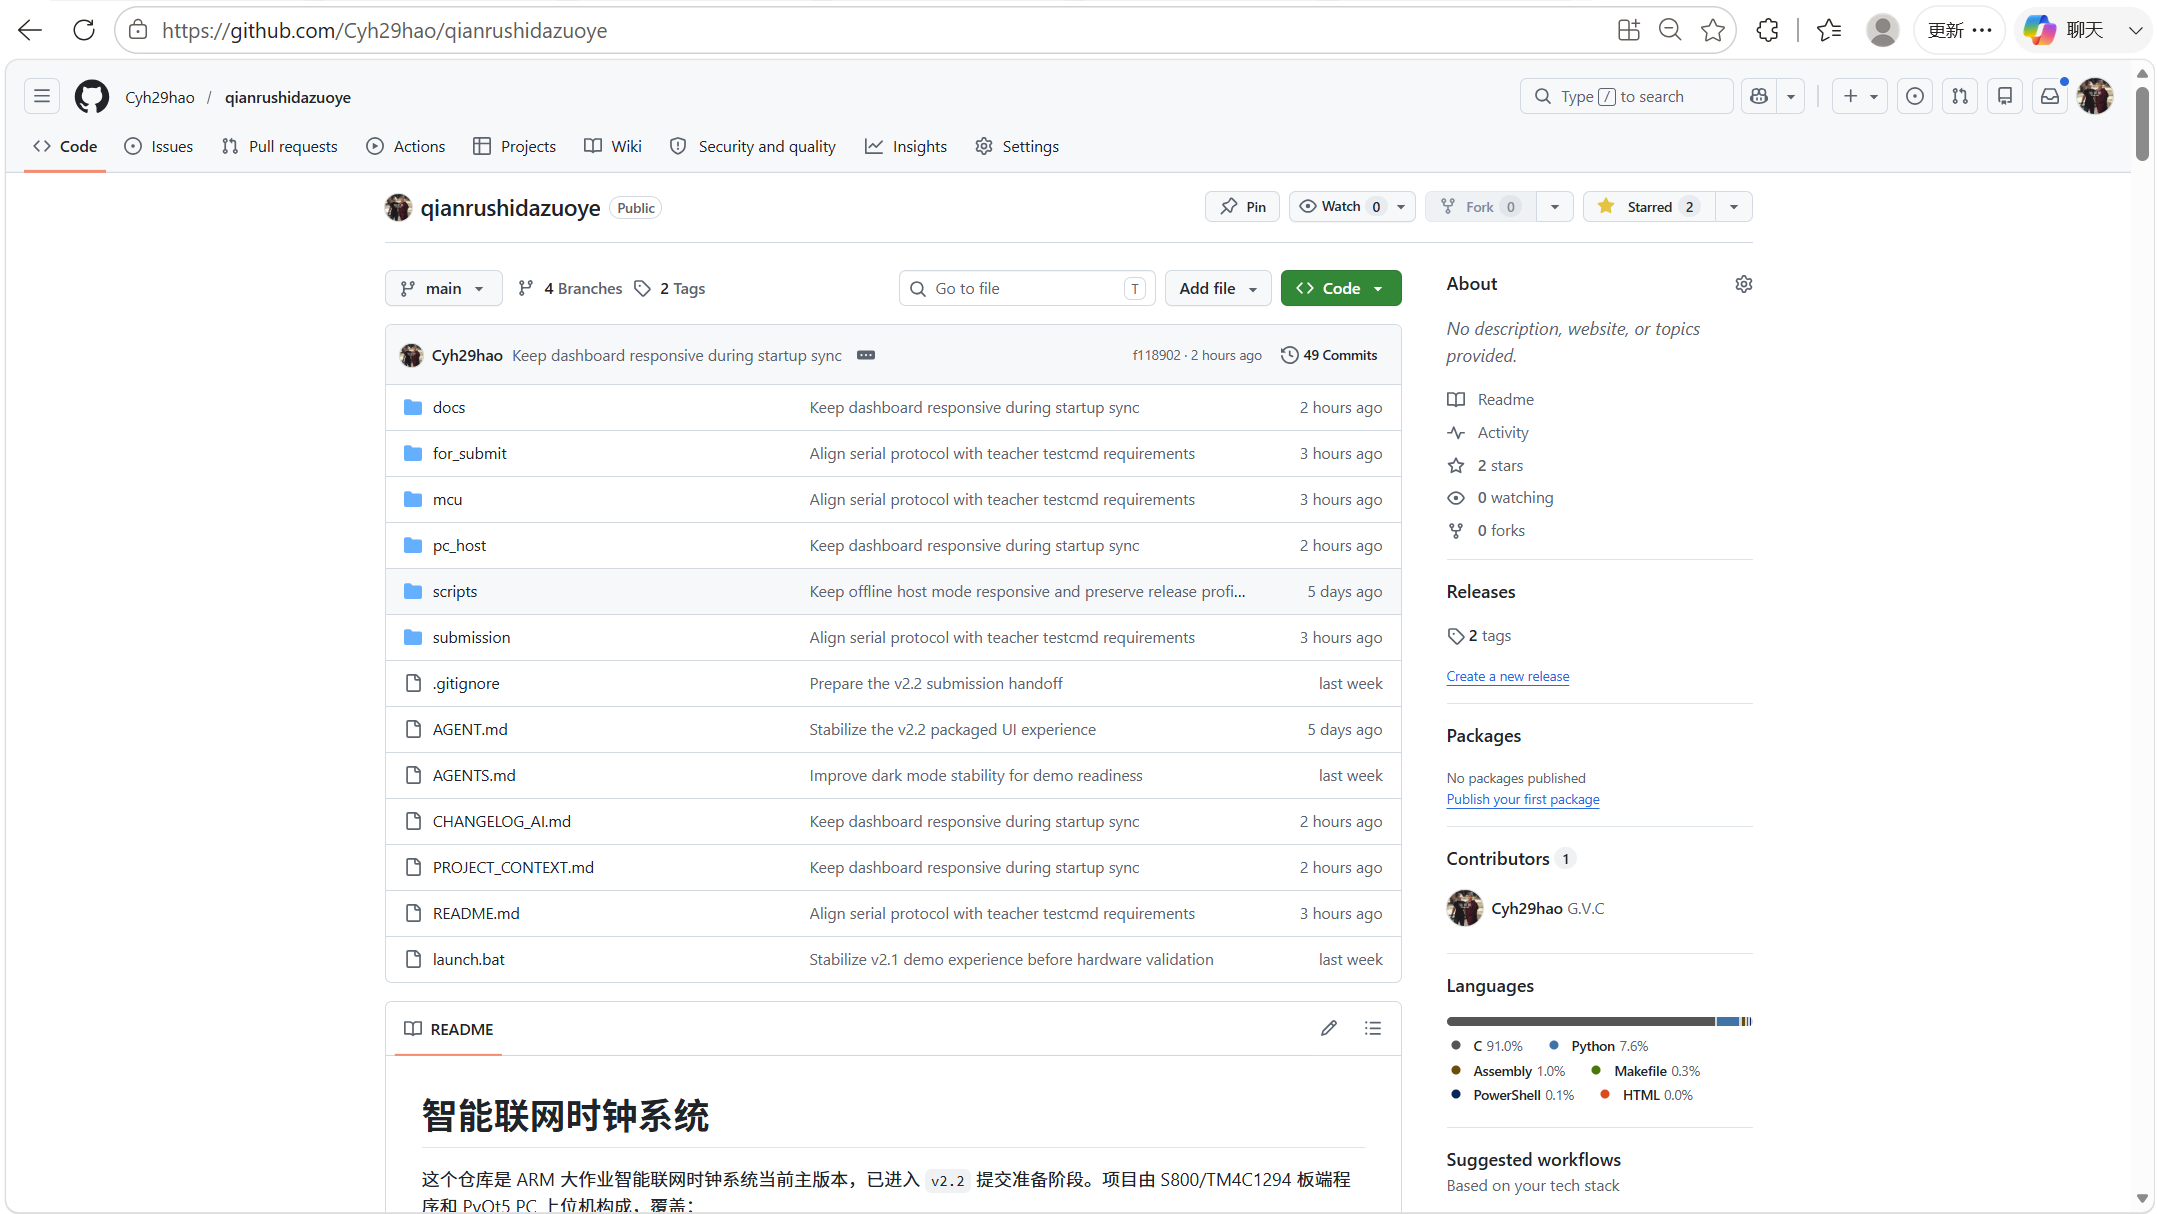
\includegraphics[width=0.96\linewidth]{github-repo.png}
\caption{GitHub 仓库页面：项目源码、文档、提交包和版本记录集中管理。}
\end{figure}

\section{测试验证与完成度}
\subsection{老师 testcmdV2.1 实板结果}
当前 v2.2 主线已按老师新发 testcmdV2.1 串口命令测试子集做过 COM5 真机复测。原始 100 条命令结果为 \keypoint{OK 92、ERROR 8、TIMEOUT 0，评分脚本 10.0/10.0}。其中 8 个 ERROR 是测试集中故意构造的非法命令，用于验证协议拒绝能力；正确行为是返回 ERROR，而不是放行非法输入。因此关键结论是合法命令无 TIMEOUT、非法命令有明确错误格式、整体评分满分。

\subsection{构建和运行验证}
MCU 端最近一次 Keil5 编译结果为 \code{0 Error(s), 0 Warning(s)}，烧录校验为 \code{Verify OK}。PC 端主要 Python 模块通过 \code{py_compile}，host-only 自动检查、COM5 quick/full 联合测试和老师协议回归均已记录在 \code{docs/} 和 \code{PROJECT_CONTEXT.md} 中。打包版 v2.2 exe/zip 已重新生成，release 目录确认不包含会覆盖用户配置的 \code{config.json}、\code{runtime_state.json}、\code{schedules.json} 或日志目录。

\begin{table}[!htbp]
\centering
\caption{主要验证证据}
\begin{tabularx}{\linewidth}{>{\bfseries}p{0.27\linewidth}X}
\toprule
验证项 & 结果\\
\midrule
MCU Keil5 构建 & 0 Error(s), 0 Warning(s)，最新固件已烧录并 Verify OK。\\
老师 testcmdV2.1 & OK 92、ERROR 8、TIMEOUT 0、评分 10.0/10.0。\\
PC 静态检查 & \code{app.py}、\code{protocol.py}、\code{twin_widgets.py}、\code{extension_services.py} 等通过 \code{py_compile}。\\
自动测试 & host-only、COM5 quick、COM5 full 覆盖 USER2、滚动消息、DISP、ERROR、高并发等项。\\
UI 检查 & 主页、系统设置、闹钟日程、调试测试、数字孪生、DAY/NIGHT 和 Matplotlib 截图检查。\\
release 打包 & SmartClockHost-v2.2.exe 和 zip 生成，保留最新 MCU 工程副本，不携带运行态配置。\\
\bottomrule
\end{tabularx}
\end{table}

\subsection{界面和交互验证}
PC 上位机曾重点修复右侧数字孪生裁切、下拉框箭头、checkbox 勾选、系统设置横向滚动、日志区拥挤、NIGHT 首启白底、菜单展开卡顿、Matplotlib 首次加载闪退风险等问题。最终界面自检覆盖普通窗口、全屏、DAY/NIGHT、四个左侧页面、右侧数字孪生、日志、底部状态栏、协议台、自动测试和 release exe 启动。后续如果继续修改 UI，项目根目录 \code{AGENT.md} 已写入硬性规则，要求右侧栏不可滚动、左侧不可被遮挡、每版修改后必须重新打包 exe 并实际运行检查。

\section{最终提交目录与运行说明}
\subsection{推荐提交结构}
最终提交包建议命名为 \code{大作业524031910102-陈云海.zip}。压缩包内部顶层目录建议包含 MCU、PC、docs、README 和必要的 release 材料。README 负责详细编译运行命令，本 PDF 负责项目说明；二者互补，不互相替代。

\noindent\textbf{推荐提交目录结构}
\begin{verbatim}
大作业524031910102-陈云海/
  mcu/
    src/main.c
    clock.uvprojx
    clock.uvoptx
    Inc/
    Driverlib/
    RTE/
    obj/s800_clock.axf
  pc_host/
    app.py
    protocol.py
    twin_widgets.py
    extension_services.py
    extension_store.py
    main.ui
    requirements.txt
    assets/
  docs/
    大作业524031910102-陈云海.pdf
    演示视频.mp4
    test-guide.md
    大作业要求逐条验收对照.md
  README.md
\end{verbatim}

\subsection{源码版和打包版启动}
源码版 PC 上位机依赖 Python、PyQt5、pyserial 和 matplotlib，可在 \code{pc_host/} 下执行 \code{launch_pc_host.ps1}。打包版为 PyInstaller onedir 程序，普通用户可直接双击 \code{build_release/SmartClockHost-v2.2/SmartClockHost.exe}。正式使用时用户配置保存在 \texttt{\%APPDATA\%/SmartClockHost-v2.2}，重新打包或替换 exe 不会抹掉已有城市、主题、日程和日志。

\subsection{教师阅读时可重点检查的现象}
如果只读文档，可以重点关注本 PDF 中的系统结构、串口协议、PC 上位机截图、扩展功能和测试证据。如果现场运行，可按“板端 RESET 开机画面 -> 板端本地按键 -> PC 连接串口自动对时 -> 数字孪生同步 -> USER1/USER2 -> 日程提醒 -> Matplotlib 看板 -> 自动测试”的顺序检查。该顺序覆盖了基础分、PC 协同、扩展功能和自主功能的主要展示点。

\section{总结}
本项目围绕课程数字时钟要求，完成了一个板端独立运行、PC 端联网增强、两端双向同步的智能联网时钟系统。MCU 端实现了时钟、日期、显示、按键、闹钟、蜂鸣、LED 和串口协议；PC 端实现了数字孪生、控制面板、日志、NTP、天气、全球时区、自动昼夜、日程、图表和自动测试。项目在实现过程中不仅关注功能是否存在，也处理了 RESET、断电重连、串口并发、NTP/天气超时、USER1/USER2 连按、跑马灯状态恢复和 UI 首启卡顿等真实联调问题。

从交付角度看，项目已经具备源码、固件工程、可运行 exe、版本管理记录、测试证据、说明文档和演示材料框架。老师不运行程序也可以通过本 PDF 理解系统设计；现场运行时，又可以通过 S800 实物、PC 数字孪生和自动测试直接验证功能闭环。这是本项目区别于普通单板时钟 demo 的主要价值。

\end{document}
